%%%%%%%%%%%%%%%%%%%%%%%%%%%%%%%%%%%%%%%%% 
% Author: Sibi <sibi@psibi.in>
%%%%%%%%%%%%%%%%%%%%%%%%%%%%%%%%%%%%%%%%% 
\documentclass{article}
\usepackage{graphicx}
\usepackage{verbatim}
\usepackage{amsmath}
\usepackage{amsfonts}
\usepackage{amssymb}
\usepackage{tabularx}
\usepackage{mathtools}
\usepackage{braket}
\usepackage[section]{placeins}
\newcommand{\BigO}[1]{\ensuremath{\operatorname{O}\bigl(#1\bigr)}}
\setlength\parskip{\baselineskip}
\begin{document}
\title{Graphs in the Plane}
\author{Sibi}
\date{\today}
\maketitle

% See here: http://tex.stackexchange.com/a/43009/69223
\DeclarePairedDelimiter\abs{\lvert}{\rvert}%
\DeclarePairedDelimiter\norm{\lVert}{\rVert}%

% Swap the definition of \abs* and \norm*, so that \abs
% and \norm resizes the size of the brackets, and the 
% starred version does not.
\makeatletter
\let\oldabs\abs
\def\abs{\@ifstar{\oldabs}{\oldabs*}}
% 
\let\oldnorm\norm
\def\norm{\@ifstar{\oldnorm}{\oldnorm*}}
\makeatother
\newpage

\section{Solution 1}

\begin{figure}[!htb]
\centering
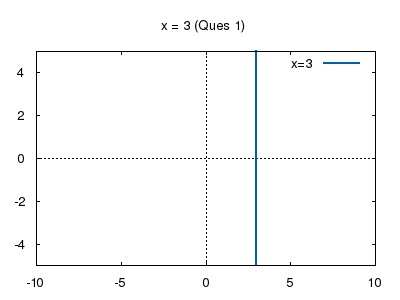
\includegraphics{./plots/one.png}
\caption{Ques 1}
\end{figure}

\section {Solution 2}

\begin{figure}[!htb]
\centering
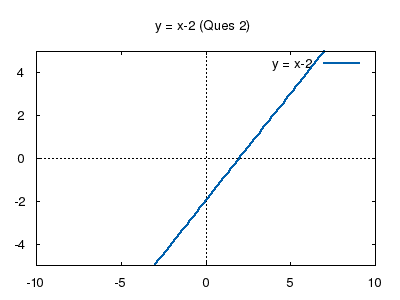
\includegraphics{./plots/two.png}
\caption{Ques 2}
\end{figure}

\section{Solution 3}

\begin{figure}[!htb]
\centering
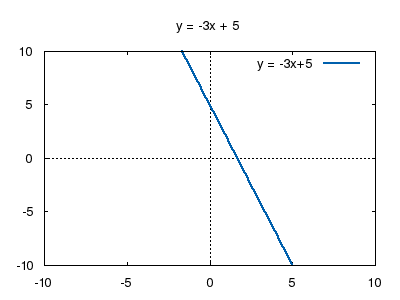
\includegraphics{./plots/three.png}
\caption{Ques 3}
\end{figure}

\end{document}

